\chapter{Implementation}\label{ch:Implementation} 
In this chapter, I will present my contributions and go over the technical aspects of the
implementation. First off, we need to discretise the theory introduced in Chapter~\ref{ch:Theory} in order
to implement the corner detection and inpainting algorithms. To do that, we need to talk about
discrete images and the method of finite differences to approximate image derivatives.
After that, we shortly talk about discretisation of diffusion processes which we need to implement
the inpainting or restoration part in order to test the mask we chose.\\  
In the second chapter I will introduce corner regions as an essential concept of this work and talk
about the additions we made to the corner detection algorithm in order to select the most valuable
corners for our inpainting mask.\\
All the source code is written in pure C and can be found in the appendix.
The initial corner detection algorithm as well as the code for the inpainting alogorithm was given
to me by courtesy of Joachim Weickert.

\section{Discretisation}\label{sec:Discretisation}
Since reality is not infinitely fine, things such as infinitesimal calculations as seen in 
calculus, e.g.\ differentation of functions, can not be applied to the real world directly.
This is a problem, because digital images are inherently not continuous as they contain only a
finite number of pixels. 
Therefore, we develop the theory in a continuous setting and then discretise it later to actually
implement the ideas as algorithms.

\subsection{Discrete Images}\label{sub:DiscreteImages}
Let $f:\Omega \rightarrow \R$ be an image where $\Omega
:= (0, n_x)\times(0, n_y) \subset \R^2$ as defined in Section~\ref{sec:Basics}. To
\textit{sample} the image, i.e.\ to discretise the image domain, we assume that all pixels lie on a
rectangular equidistant grid inside $\Omega$, where each cell in the grid has a size of $h_x
\times h_y$.\newpage\noindent
That yields $N_x := n_x/h_x$ pixels in x- and $N_y := n_y/h_y$ pixels in
y-direction.
That being said, we define the pixel $u_{i,j}$ at grid location ${(i, j)}^\top$ as
\begin{equation}
    u_{i, j} := u(ih_x, jh_y)\qquad \forall(i ,j) \in \{1,\dots,N_x\}\times\{1,\dots,N_y\}
\end{equation}
With that approach, the pixels are defined to lie on the crossing of the grid lines.
An alternative idea defines the pixels to lie in the centre of each cell, i.e.\ at location 
\begin{equation}
    {\left(\left(i-\frac{1}{2}\right)h_x,\ \left(j- \frac{1}{2}\right)h_y\right)}^\top
\end{equation}
As a sidenote, the cell sizes in either direction are almost always assumed to be 1 in 
practice. 
To keep the theory as universal as possible, however, we will use $h_x$ and $h_y$ instead.\\
Sampling of the spatial domain is not the only step necessary to fully discretise an image. We also have
to discretise the \textit{co-domain} or \textit{grey-value-domain}. This step of
the discretisation process is also called \textit{quantisation}. In the continuous setting, the so
called \textit{co-domain} is the complete set of irrational numbers $\R$. To save disk space, this
range is usually limited to 1 byte, that is values in the range of whole numbers from 0 to
$2^8=256$~\cite{ipcv}.

\subsection{Numerical Differentiation}\label{sub:NumDiff}
Image derivatives are essential to image processing as seen in the previous chapter. 
Therefore, we need a way to compute them even on discrete images. To compute the 
gradient or, in the simpler case, the derivative of a discrete function, one 
generally uses so called \textit{finite difference schemes}. 
Such a scheme is normally derived from the \textit{Taylor expansion} of the continuous
function. For example, we want to compute the first derivative of a 1D function $f:\R
\rightarrow \R$.
The Taylor expansion of \textit{degree $n$} of this function around the point $x_0\in\R$ is given by 
\begin{equation}
    f(x) = T_n(x, x_0) + \mathcal{O}(h^{n+1})
\end{equation}
where $\mathcal{O}(h^{n+1})$ describes the magnitude of the leading error term and as such the
\textit{approximation quality} of the Taylor series.
The actual Taylor series is defined as
\begin{equation}
    T_n(x, x_0) = \sum\limits_{k=0}^{n} \frac{{(x-x_0)}^k}{k!}f^{(k)}(x_0)
\end{equation}
where $f^{(k)}$ denotes the $k$-th derivative of the function $f$.\newpage\noindent
A finite difference scheme generally uses a weighted sum of neighbouring values to compute the
desired derivative expression. In our example, we want to derive a scheme to compute the first
derivative of $f_i$ using its neighbours $f_{i-1}$ and $f_{i+1}$, i.e.
\begin{equation}
    f_i' \approx \alpha f_{i-1} + \beta f_i + \gamma f_{i+1}
\end{equation}
We can now describe $f_{i-1}$ and $f_{i+1}$ in terms of their Taylor expansion around $f_i$: 
\begin{align}
    f_{i-1} &= f((i-1)h) \notag\\
            &= T_n((i-1)h, ih) + \mathcal{O}(h^{n+1})\notag\\
            &= \sum\limits_{k=0}^{n}\frac{{(-h)}^k}{k!}f_i^{(k)}+ \mathcal{O}(h^{n+1})\\
    f_{i+1} &= \cdots = \sum\limits_{k=0}^{n}\frac{h^k}{k!}f_i^{(k)}+ \mathcal{O}(h^{n+1})
\end{align}
If we now choose a concrete value for $n$ (here $n=5$) we can actually compute the approximation:
\begin{align}
    f_{i-1} &= f_i - hf_i' + \frac{h^2}{2}f_i'' - \frac{h^3}{6}f_i^{(3)} + \frac{h^4}{24}f_i^{(4)} -
    \frac{h^5}{120}f_i^{(5)} + \mathcal{O}(h^6)\label{eq:fi-1}\\
    f_{i+1} &= f_i + hf_i' + \frac{h^2}{2}f_i'' + \frac{h^3}{6}f_i^{(3)} + \frac{h^4}{24}f_i^{(4)} +
    \frac{h^5}{120}f_i^{(5)} + \mathcal{O}(h^6)\label{eq:fi+1}
\end{align}
The next step is the \textit{comparison of coefficients}. We insert~\eqref{eq:fi-1} and~\eqref{eq:fi+1}
into the equation and solve the arising linear system of equations for $\alpha,\beta,\gamma$.
\begin{align}
    0\cdot f_i + 1\cdot f_i' + 0\cdot f_i'' \overset{!}{=} \alpha f_{i-1} + \beta f_i + \gamma
    f_{i+1}
\end{align}
After the substitution, the right hand side becomes
\begin{align}
    &\alpha \left(f_i - hf_i' + \frac{h^2}{2}f_i''\right) + \beta f_i + \gamma\left(f_i + hf_i' + \frac{h^2}{2}f_i''\right)\notag\\
    = &\left(\alpha+\beta+\gamma\right)f_i + h\left(-\alpha+\gamma\right)f_i' + \frac{h^2}{2}\left(\alpha+\gamma\right)f_i''
\end{align} 
Note that for the comparison of coefficients it suffices to use the first 3 summands of the
approximation.\newpage\noindent
The linear system defined by the above equation
\begin{equation}
    \begin{pmatrix}
        1&1&1\\
        -1&0&1\\
        1&0&1
    \end{pmatrix}
    \begin{pmatrix}
        \alpha\\
        \beta\\
        \gamma
    \end{pmatrix}
    =
    \begin{pmatrix}
        0\\
        \frac{1}{h}\\
        0
    \end{pmatrix}
\end{equation}
has the solutions $\alpha = -\frac{1}{2h}, \beta = 0, \gamma = \frac{1}{2h}$.
This yields the approximation 
\begin{equation}
    f_i'\approx\frac{f_{i+1} - f_{i-1}}{2h}
\end{equation}
To find out how good this scheme is, we re-insert~\eqref{eq:fi-1} and~\eqref{eq:fi+1} to get
\begin{align}
    \frac{f_{i+1} - f_{i-1}}{2h}= -&\frac{1}{2h}\left(f_i - hf_i' + \frac{h^2}{2}f_i'' -
        \frac{h^3}{6}f_i^{(3)} + \frac{h^4}{24}f_i^{(4)} -
    \frac{h^5}{120}f_i^{(5)} + \mathcal{O}(h^6)\right) + \notag\\
                                   &\frac{1}{2h}\left(f_i - hf_i' + \frac{h^2}{2}f_i'' -
                                       \frac{h^3}{6}f_i^{(3)} + \frac{h^4}{24}f_i^{(4)} -
                                   \frac{h^5}{120}f_i^{(5)} + \mathcal{O}(h^6)\right)\notag
\end{align}
Expanding and simplifying yields
\begin{align}
        \frac{f_{i+1} - f_{i-1}}{2h} &= f_i' + \underbrace{\frac{h^2}{6}f_i'' +
            \frac{h^4}{30}f_i^{(4)} +
        \mathcal{O}(h^5)}_\text{quadratic leading error term}\notag\\
            \Rightarrow \frac{f_{i+1} - f_{i-1}}{2h} &= f_i' + \mathcal{O}(h^2)
\end{align}
This means that the error of our approximation is quadratic in the grid size. 
We also say that this approximation has a \textit{consistency order} of 2. Note that for such an
approximation to be reasonable, it has to have at least consistency order of 1. Otherwise, it is
not guaranteed that the error term diminishes if we send the grid size $h$ to 0.\\
The scheme derived above is also called \textit{central difference scheme}. Note that there are
other schemes such as \textit{forward} and \textit{backward} differences, but for the most part, we
will only use central differences since it provides us with the highest consistency
order out of all three. 
\begin{align}
    f_i' &= \frac{f_i - f_{i-1}}{h} + \mathcal{O}(h)&\textnormal{(backward differences)}\notag\\
    f_i' &= \frac{f_{i+1} - f_i}{h} + \mathcal{O}(h)&\textnormal{(forward differences)}\notag
\end{align}
\newpage\noindent
\subsection{Numerical Schemes for Diffusion}\label{sub:NumSchemesDiffusion}
As discretisation for the inpainting process, the non-standard discretisation scheme as
derived in~\cite{www13} was used. The actual derivation of the scheme is fairly complex 
and beyond the scope of this thesis.
That is why I will just cover the essential information and then refer the interested 
reader to~\cite{weickert96, www13} for more information on numerical schemes for diffusion
processes in general.\\
We remember the defining equation of EED\@:
\begin{equation}
    \partial_t u = \diverg(\underbrace{g(\del u_\sigma\del u_\sigma^\top)}_{=:D}\del
    u)\label{eq:EED}
\end{equation}
To discretise this equation, we first write the diffusion tensor $D$ as a symmetric matrix
\begin{equation}
    D = \begin{pmatrix}
        a&b\\b&c
    \end{pmatrix}
\end{equation}
Resubstituting this into~\eqref{eq:EED}, we get 
\begin{equation}
\partial_t u = \diverg \begin{pmatrix}
    a\cdot \partial_x u+b\cdot \partial_y u\\
    b\cdot \partial_x u+c\cdot \partial_y u
\end{pmatrix} = a\cdot\partial_{xx} u + 2b\cdot \partial_{xy}u+ c\cdot \partial_{yy} u
\end{equation}
These second order derivatives can easily be discretised using central differences. This leads to a
fairly complex stencil that the interested reader can look up in~\cite{weickert96}.
The problem with this discretisation is that it is not guaranteed to satisfy the
\textit{nonnegativity requirement} or \textit{stability in the maximum norm}~\cite{weickert96}. This requirement is
an important theoretical requirement as it is needed to guarantee the well-posedness of the
diffusion process, which in turn guarantees the numerical stability of the
algorithm~\cite{weickert96}.
In order to enable the discretisation to fulfill this requirement, one has to impose the restriction that
the \textit{spectral condition number $\kappa$}, which is the ratio between the smallest and
largest eigenvalue of the matrix $D$, is bounded by 
\begin{equation}
    \kappa \leq 3 + 2\sqrt{2}
\end{equation}
This restriction might seem arbitrary, but the proof of this upper bound can be found
in~\cite{weickert96}.
However, this requirement also puts a restriction on the anisotropy of the diffusion process, as the
ratio between the largest and smallest eigenvalue of the diffusion tensor is now bounded from above.
Therefore, one might consider another discretisation that is not necessarily stable in
the maximum norm.\newpage\noindent
In~\cite{www13}, a whole framework for discretisations stable in the
\textit{euclidean or 2-norm} was derived. This framework embeds a series of 8 different
stencils that are dependent on 2 parameters $\alpha, \beta$. Let us now denote such a spatial
discretisation of~\eqref{eq:EED} by 
\begin{equation}
    \frac{d\mathbf{u}}{dt} = \mathbf{A}(\mathbf{u})\mathbf{u}
\end{equation}
It can be shown that the matrix $\mathbf{A}$ is negative semidefinite, i.e.\  
\begin{equation*}
    x^\top \mathbf{A}x \leq 0
\end{equation*}
for all vectors $x$, if the parameters $\alpha,\beta$ satisfy
\begin{eqnarray}
    0 \leq \alpha \leq \frac{1}{2}\\
    \vert\beta\vert \leq 1-2\alpha
\end{eqnarray}
The negative semidefiniteness of $\mathbf{A}$ is useful to show that the semi-implicit and
explicit time discretisations both are stable in the 2-norm.
Both time discretisations work by applying a forward difference on
the temporal derivative on the left side with a time step size $\tau$ (this corresponds to the grid
size in the spatial derivative). 
The difference between the explicit and the implicit time discretisation is fairly small, but makes
a huge difference in efficiency since, as we will see next, we can choose much larger time steps in
the semi-implicit scheme than in the explicit scheme. 
The difference lies in the fact, that in the explicit scheme, the right hand side does not involve any terms
`from the future', while in the semi-implicit scheme it does.
We can now write the explicit scheme given by
\begin{equation}
    \frac{u^{k+1} - u^{k}}{\tau} = \mathbf{A}(u^k)u^k
\end{equation}
as
\begin{equation}
    u^{k+1} = (I + \tau\mathbf{A}(u^k))u^k
\end{equation}
The upper index $k$ denotes the `time level' of $u$.
Stability for this scheme can be guaranteed, if 
\begin{equation}
    \rho(I + \tau\mathbf{A}(u^k)) \leq 1\ \Leftrightarrow\ \tau \leq \frac{2}{\rho(\mathbf{A}(u^k))}
\end{equation}
where $\rho$ denotes the \textit{spectral norm} or \textit{modulus of the largest
eigenvalue}~\cite{www13}.\newpage\noindent
The semi-implicit scheme, however, is given by
\begin{equation}
    \frac{u^{k+1} - u^{k}}{\tau} = \mathbf{A}(u^k)u^{k+1}
\end{equation}
which boils down to solving the linear system of equations
\begin{equation}
    (I-\mathbf{A}(u^k))u^{k+1} = u^k\label{eq:SemiImpl}
\end{equation}
Note that the matrix on the left hand side is invertible thanks to the negative semidefiniteness of
$\mathbf{A}(u^k)$: One can show that because of the negative semidefiniteness, $(I-\mathbf{A}(u^k))$ only has eigenvalues
larger than 1.
This shows that the semi-implicit scheme given by 
\begin{equation}
    u^{k+1} = {(I- \mathbf{A}(u^k))}^{-1}u^k
\end{equation}
is stable in the 2-norm for every time step size $\tau$.\\
Furthermore, in the semi-implicit scheme the next iteration can not be computed explicitly (as the name
suggests) as is the case with the explicit scheme. Instead one has to solve
the linear system of equations given by~\eqref{eq:SemiImpl}. This is usually done with an iterative
solver like Gauss-Seidel or conjugate gradients (CG)~\cite{conjugateGradients}. 
An in-depth explanation of these solvers would be beyond the scope of this thesis.
The only thing important to know is that for the evaluation of the inpainting masks in my thesis,
I used a semi-implicit scheme with a conjugate gradients solver and a timestep size of 1000.

\section{Circular Corner Regions}\label{sec:Contribution}
As mentioned in the beginning, the main concern for the approach of Zimmer~\cite{zimmer07} was that the 
corner localisation was not accurate enough that we can just keep a 4 or 8-neighbourhood 
of pixels. The implication is that the regions they inserted into the mask were were too small to
cover the potential uncertainty in the corner localisation process stemming from the Gaussian
smoothing in the computation of the structure tensor (see~\ref{sec:Structure}). Specifically
because in order to limit the amount of corners detected, they chose to vary the integration scale
parameter increasing the uncertainty in the localisation, this poses a problem.\newpage\noindent
Hence, I want to explore increasing the neighbourhood of pixels that is kept around each
corner. A disk-shaped neighbourhood with radius $r$ and origin point $(x, y)$ (also called a
\textit{(circular) corner region} in the following) is defined as 
\begin{equation}
    B_r(x, y) = \lbrace (x',y') \in \Omega\ \vert\ {(x'-x)}^2 + {(y'-y)}^2 \leq r^2\rbrace
\end{equation}
The optimal choice for the radius of the corner disks is discussed in
Section~\ref{sec:ParameterSelection}.
Increasing the radius of the corner regions obviously leads to denser masks if one does not adjust
the limit of corner regions that are put in the mask. Since doing this manually for every picture
would not be practical at all in the context of a codec, we have to come up with a way to make sure
the resulting masks are always similar in pixel density.\\
One way to achieve this would be to introduce a percentile parameter instead of using the constant
threshold from the corner detection method described in~\ref{sub:Corner}.

\subsection{Percentile Thresholding}\label{sub:Percentile}
In the classic version of Harris corner detection, an artificial threshold parameter $T$
is introduced to weed out `bad' corners, i.e.\ corners where the \linebreak 
Harris measure~\eqref{def:Harris} is low. 
This parameter, however, is fairly sensible to the input image.\\
As a workaround to make this parameter a bit more robust, a percentile
parameter is introduced that is in turn used to compute a more robust threshold.\\
In statistics, the \textit{n-th percentile} of a set is the value that is larger than $n$ percent
of all values in this set.
I computed the percentile using the \textit{nearest-rank method} since this was the easiest
approach and worked good enough already. In this method, the n-th percentile is just simply
computed as the value at position 
\[
\lceil \frac{n}{100}\cdot N_{x}N_{y}\rceil
\] 
of the ordered set of values~\cite{percentile}.\\
Since in an image, there are more non-corners than actual corners, we have to deal with many zero
or close-to-zero cornerness values. This is a problem because the percentile computation would be skewed
heavily if e.g.\ more than 80 percent of all values are zero already. To solve this, I first filtered
out all values below a threshold close to zero and then accumulated the remaining values into an
array of appropriate size. This array is then sorted using an already implemented Quicksort
algorithm from the C standard library.\\
Subsequently, the new threshold is given as the value at
the index calculated above.
%\begin{figure}[ht]
    %\lstinputlisting[language=C, linerange={664-670,675-703}]{/home/daniel/Uni/Thesis/src/corner_detection.c}
    %\caption{Total pixel percentage thresholding}
%\end{figure}\\
While this approach works a bit better than the original version using the fixed threshold, it is
still not perfect. For example, if one uses a percentile of $0.5$, meaning that 
$50\%$ of all corners are thrown out, one could still get wildly different results 
for two different input images as we can see in~\ref{fig:PercExample}.
\begin{figure}[h!]
    \centering
    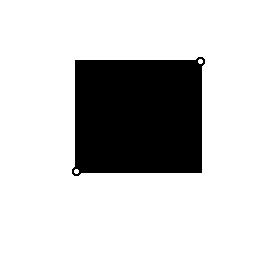
\includegraphics[width=0.4\linewidth]{example_rect_50.png}
    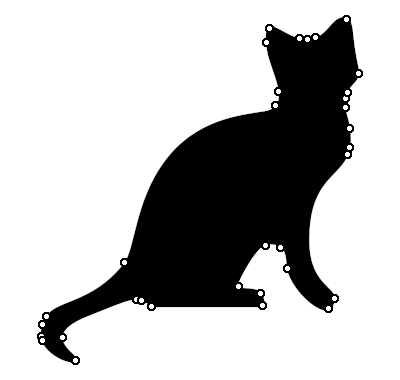
\includegraphics[width=0.4\linewidth]{example_cat_50.png}
    \caption{Corner detection with the same parameters. Parameters are $\sigma=1,\rho=2,q=0.3$, no
    CNMS, no TPPT}
    \label{fig:PercExample}
\end{figure}\\
To tackle this issue, I propose a new method that I call \textit{Total Pixel Percentage
Thresholding}. The idea behind this method is that one makes the amount of corners that are kept
in the masks dependent on the mask radius, i.e.\ the radius of a corner region in the inpainting
mask. In other words, one specifies the desired mask pixel density and depending on the mask
radius, the maximum number of corners that can be inserted into the mask is
calculated.
The problem of calculating the number of pixels inside a disc of radius $r$ is also known as
\textit{Gauss' circle problem}~\cite{gaussCircle}. The exact solution to this problem is given
by~\cite{hilbert96}
\begin{equation}
    N(r) = 1 + 4\sum_{i=0}^{\infty}\left(\left\lfloor\frac{r^2}{4i+1}\right\rfloor - \left\lfloor
    \frac{r^2}{4i+3}\right\rfloor\right)
\end{equation}
but since this is an infinite sum, the exact solution can not be computed this way. This is why I
chose the naive way by just iterating through a loop and count the numbers inside the disk.
I could have also chosen to use an upper bound and estimate the number of pixels that 
way, but this would not have been as accurate.\\
%\begin{figure}[ht]
    %\centering
    %\lstinputlisting[language=C, linerange={424-435}]{/home/daniel/Uni/Thesis/src/utils.c}
    %\caption{Computation of number of pixels in disk}\label{fig:PixelRegion}
%\end{figure}
\newpage\noindent
After computing the area per corner region we can simple calculate how many regions can be inserted
into the mask without exceeding the pixel density threshold by the equation
\begin{equation}
    N_{corners} = \left\lceil \frac{q \cdot N_{x}N_{y}}{N_{disc}} \right\rceil,\qquad0\leq q\leq 1 
\end{equation}
where $q$ is the percentile parameter, $N_x, N_y$ the number of pixels in the respective direction
and $N_{disc}$ the amount of pixels per corner region. $N_{corners}$ is then an upper bound on the
amount of corners.
Using this method, the pixel density of inpainting masks can be consistently recreated, as we will
see in the next chapter where I will present some examples of this method in action.\\
Note that I did not consider the potential overlap of corner regions inside the
computation of this upper bound, since there would have been no easy way to determine the amount of
overlapping pixels a priori.
Instead, I introduced another method tackling the issue of potentially overlapping corner regions
called \textit{Circular non-maximum suppression}. We will see how this method
works in the next Section~\ref{sub:Suppression}.
Another thing to mention is that the amount of pixels in the mask using this approach is limited by
the number of corners detected since I do not even consider pixels that have a sufficiently small
cornerness value as mask candidates.
\newpage
\subsection{Circular Non Maximum Suppression}\label{sub:Suppression}
\begin{figure}[t]
    \begin{lstlisting}[language=Python]
# Circular non-maximum suppression at x with radius r.
# Parameters:
#    -harris: Harris measure map
#    -x: current location as tuple
#    -r: radius of corner regions
#    -out: map of accepted corners after suppression
def circular_suppression(harris, x, r, out):
    for y in circle(x, r):
        if harris[y] > harris[x]:
            # The current location is not a maximum
            out[x] = 0
            return
    # Current location is a maximum, keep the region around it
    out[x] = harris[x]
    \end{lstlisting}
    \caption{Pseudo-Code for circular non-maximum suppression}
\end{figure}
\noindent As mentioned previously, overlapping corner regions tend to worsen the estimation of the mask pixel
density. 
Furthermore, as Zimmer already stated in~\cite{zimmer07} the sparsity of corners in images poses a
problem for the reconstruction quality. This method is supposed to tackle both of these issues by
increasing the radius of the local maximum search during the corner detection. In the original
corner detection method, corners are determined by the local maxima inside an 
8-neighbourhood of the cornerness measure. The idea is to adapt the radius of the neighbourhood for the
local maximum search to the mask radius. As experiments showed (see Section~\ref{sec:Results}), this minimises the overlap in
corner regions in the final mask and enables a fairly accurate estimation of the mask pixel
density, allowing us to consistently produce masks with similar density. \\
The other issue that this method tries to solve is the uneven distribution of corners across
the whole image. \\
When limiting the amount of corners that are selected into the mask, one should not only care about
the `cornerness' of a corner, but also about its position. In other words, if a lot of good corners
are in close proximity to each other, it would be better to choose the ones that encase the 
highest number of `good' corners around them. 
That way, we get multiple corners `for the price of one' and can still introduce some 
of the `worse' corners to the mask.
By minimising the overlap between corner regions through this circular non-maximum suppression, we
can actually eliminate corners that are already covered by another disk from `a better' corner and
thus free up some slots for corners that may otherwise not have been selected for being sub-par.\\
One should note that this is not a perfect solution as certain constellations of corners create
a corner case in which a corner that is assumed to cover another corner is removed for being in the
disk of a better corner. This leads to the case where the corner that was formerly assumed to be
covered is suddenly not covered anymore and disappears from the mask without replacement, so future
work might be invested into finding a better solution for this approach.

